\documentclass{article}
\usepackage[utf8x]{inputenc}
\usepackage{ucs}
\usepackage{amsmath} 
\usepackage{amsfonts}
\usepackage{upgreek}
\usepackage[english,russian]{babel}
\usepackage{graphicx}
\usepackage{float}
\usepackage{textcomp}
\usepackage{hyperref}
\usepackage{geometry}
  \geometry{left=2cm}
  \geometry{right=1.5cm}
  \geometry{top=1cm}
  \geometry{bottom=2cm}
\usepackage{tikz}
\usepackage{ccaption}
\usepackage{multicol}


\usepackage{listings}


\begin{document}
\pagestyle{plain}
\lstset{
  language=C,                % choose the language of the code
  basicstyle=\linespread{1.1}\ttfamily,
  columns=fixed,
  fontadjust=true,
  basewidth=0.5em,
  keywordstyle=\color{blue}\bfseries,
  commentstyle=\color{gray},
  stringstyle=\ttfamily\color{orange!50!black},
  showstringspaces=false,
  numbersep=5pt,
  numberstyle=\tiny\color{black},
  numberfirstline=true,
  stepnumber=1,                   % the step between two line-numbers.        
  numbersep=10pt,                  % how far the line-numbers are from the code
  backgroundcolor=\color{white},  % choose the background color. You must add \usepackage{color}
  showstringspaces=false,         % underline spaces within strings
  captionpos=b,                   % sets the caption-position to bottom
  breaklines=true,                % sets automatic line breaking
  breakatwhitespace=true,         % sets if automatic breaks should only happen at whitespace
  xleftmargin=.2in,
  extendedchars=\true,
  keepspaces = true,
}
\lstset{literate=%
   *{0}{{{\color{red!20!violet}0}}}1
    {1}{{{\color{red!20!violet}1}}}1
    {2}{{{\color{red!20!violet}2}}}1
    {3}{{{\color{red!20!violet}3}}}1
    {4}{{{\color{red!20!violet}4}}}1
    {5}{{{\color{red!20!violet}5}}}1
    {6}{{{\color{red!20!violet}6}}}1
    {7}{{{\color{red!20!violet}7}}}1
    {8}{{{\color{red!20!violet}8}}}1
    {9}{{{\color{red!20!violet}9}}}1
}

\title{Семинар \#7: Структуры. Классные задачи.\vspace{-5ex}}\date{}\maketitle

\section*{Часть 1: Основы структур}

Структуры служат для объединения нескольких типов в один. В примере ниже был создан новый тип под названием \texttt{struct point}. Переменные этого типа будут содержать внутри себя 2 значения типа \texttt{float}.
\begin{lstlisting}
#include <stdio.h>

struct point {
    float x, y;
}; // <--------------------------- Не забудьте тут точку с запятой!

int main() {
    struct point a = {2.1, 4.3};
    a.x = 7.8;
    printf("(%f, %f)", a.x, a.y);
}
\end{lstlisting}

\subsection*{Операции со структурами}
\begin{enumerate}
\item При создании структуры её элементы можно инициализировать с помощью фигурных скобочек.
\begin{lstlisting}
struct point a = {2.1, 4.3};
\end{lstlisting}
Однако нельзя таким образом присваивать
\begin{lstlisting}
a = {5.6, 7.8}; // Ошибка, фигурными скобочками можно только инициализировать!
\end{lstlisting}
\item Доступ к элементу структуры осуществляется с помощью оператора точка
\begin{lstlisting}
a.x = 5.6;
a.y = 7.8;
\end{lstlisting}
\item Структуры можно присваивать друг другу. При этом происходит побайтовое копирование содержимого одной структуры в другую.
\begin{lstlisting}
struct point b;
b = a;
\end{lstlisting}
\end{enumerate}

\subsection*{Массив структур}
Структуры, как и обычные переменные, можно хранить в массивах. В примере ниже создан массив под названием \texttt{array}, содержащий в себе 2 точки.
\begin{lstlisting}
#include <stdio.h>
struct point {
    float x, y;
};
int main() {
    struct point array[3] = {{2.1, 4.3}, {7.0, 3.1}, {1.5, 0.2}};
    array[1].x = 1.8;
    printf("(%f, %f)", array[0].x, array[0].y);
}
\end{lstlisting}

\subsection*{Передача структуры в функцию}
Структуры можно передавать в функции и возвращать из функций также как и обычные переменных. При передаче в функцию происходит полное копирование структуры и функция работает уже с копией структуры. При возвращении из функции также происходит копирование.
\begin{lstlisting}
#include <stdio.h>
struct point {
    float x, y;
};
void print_point(struct point a) {
    printf("(%f, %f)", a.x, a.y);
}
struct point add_points(struct point a, struct point b) {
    struct point result;
    result.x = a.x + b.x;
    result.y = a.y + b.y;
    return result;
}
int main() {
    struct point a = {2.1, 4.3}, b = {6.7, 8.9};
    struct point c = add_points(a, b);
    print_point(c);
}
\end{lstlisting}
\vspace*{-\baselineskip}
\subsection*{Структуры содержащие более сложные типы данных}
Структуры могут содержать в себе не только базовые типы данных, но и более сложные типы, такие как массивы (в том числе строки), указатели, а также другие структуры.\\
Пример программы, в которой описывается структура для удобной работы с объектами Книга (\texttt{struct book}).
\begin{lstlisting}
#include <stdio.h>
#include <string.h>
struct book {
    char title[50];
    int pages;
    float price;
};
void print_book(struct book b) {
    printf("Book info:\n");
    printf("Title: %s\nPages: %d\nPrice: %g\n\n", b.title, b.pages, b.price);
}
int main() {
    // Создаём книгу:
    struct book a = {"The Martian", 10, 550.0};
    
    // Меняем количество страниц книги и её название и печатаем её
    a.pages = 369;
    strcpy(a.title, "The Catcher in the Rye");
    print_book(a);
    
    // Пример работы с массивом структур
    struct book scifi_books[10] = {{"Dune", 300, 500.0}, {"Fahrenheit 451", 400, 700.0},
							 {"Day of the Triffids", 304, 450.0}};
    scifi_books[2].price = 2000.0;
    print_book(scifi_books[2]);
}
\end{lstlisting}
\newpage
\section*{Часть 3: Указатели на структуры:}
Указатель на структуру хранит адрес первого байта структуры. Для доступа к полям структуры по указателю нужно сначала этот указатель разыменовать, а потом использовать: \texttt{(*p).price}. Для удобства был введён оператор стрелочка \texttt{->}, который делает то же самое: \texttt{p->price}.
\begin{multicols}{2}
\begin{lstlisting}
#include <stdio.h>

struct book {
    char title[50];
    int pages;
    float price;
};
int main() {
    struct book a = {"The Martian",277,540};
    struct book* p = &a;
    
    // Три способа доступа к полю:
    a.price += 10;
    (*p).price += 10;
    p->price += 10;
}
\end{lstlisting}

\vfill\null
\columnbreak

\vspace*{3\baselineskip}
\begin{center}
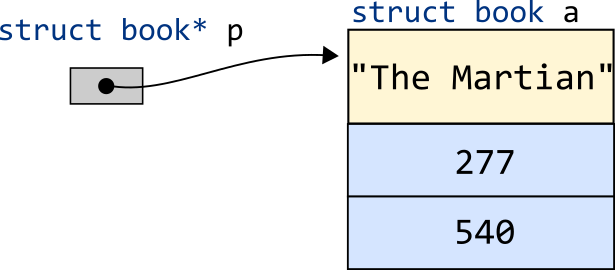
\includegraphics[scale=0.5]{../images/structpointer2.png}
\end{center}
\end{multicols}


\subsection*{Передача по значению}
При обычной передаче в функцию всё содержимое копируется. Функция работает с копией.
\begin{lstlisting}
#include <stdio.h>
struct book {
    char title[50];
    int pages;
    float price;
};
void change(struct book a) {
    a.price += 10;
}
int main() {
    struct book a = {"The Martian",277,540};
    change(a); // внутри функции структура a НЕ изменится
}
\end{lstlisting}
\begin{center}
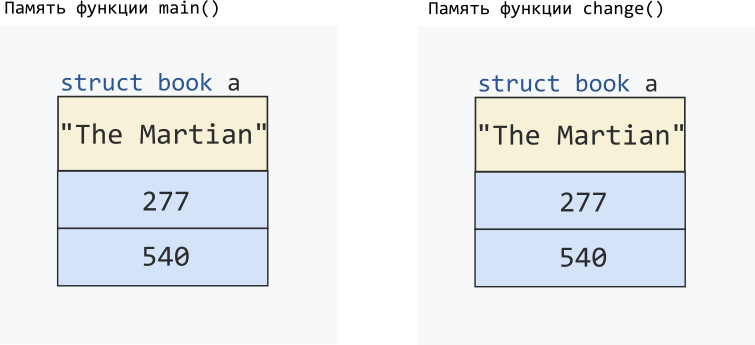
\includegraphics[scale=0.6]{../images/structpassbyvalue.png}
\end{center}


\subsection*{Передача по указателю}
При передаче в функцию по указателю копируется только указатель.
\begin{lstlisting}
#include <stdio.h>
struct book {
    char title[50];
    int pages;
    float price;
};
void change(struct book* p) {
    p->price += 10;
}
int main() {
    struct book a = {"The Martian",277,540};
    struct book* p = &a;
    change(p); // внутри функции структура a изменится
}
\end{lstlisting}
\begin{center}
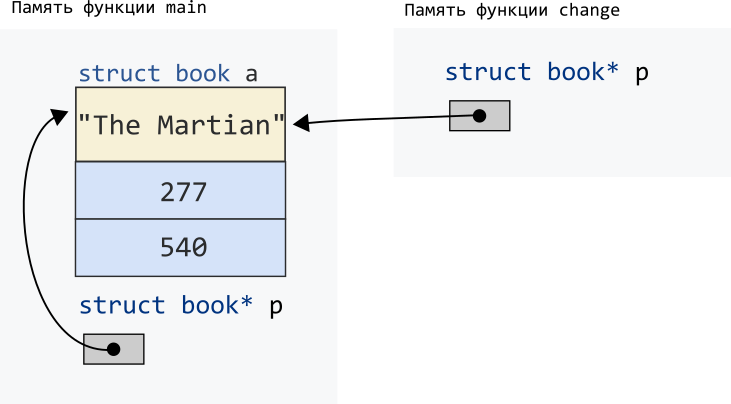
\includegraphics[scale=0.6]{../images/structpassbypointer.png}
\end{center}
Такой способ передачи имеет 2 преимущества:
\begin{enumerate}
\item Можно менять структуру внутри функции, и изменения будут действительны вне функции
\item Не приходится копировать структуры, поэтому программа работает быстрее.
\end{enumerate}

\subsection*{Передача по указателю на константу}
Иногда мы не хотим менять структуру внутри функции, но хотим чтобы ничего не копировалось. Тогда желательно использовать передачу по указателю
на константу.
\begin{lstlisting}
#include <stdio.h>
struct book {
    char title[50];
    int pages;
    float price;
};
void print_book_info(const struct book* p) {
    printf("Title: %s\nPages: %d\nPrice: %g\n\n", p->title, p->pages, p->price);
}
int main() {
    struct book a = {"The Martian",277,540};
    print_book_info(&a);
}
\end{lstlisting}
\newpage


\newpage
\section*{Часть 4: Выравнивание}
Пусть есть структура \texttt{struct test} и нам нужно узнать её размер если размеры типов \texttt{char}, \texttt{int} и \texttt{double} равны \texttt{1}, \texttt{4} и \texttt{8} байт соответственно.
\begin{lstlisting}
struct test {
    int a;
    char b;
    double c;
};
\end{lstlisting}
Кажется, что размер этой структур равен сумме размеров состовляющих её элементов, то есть \texttt{13}. Но это не так. 
На самом деле размер этой структуры будет отличаться в зависимости от вычислительной системы, на которой запускается код (как, впрочем, и размеры других типов). Но на большинстве вычислительных систем размер структуры \texttt{struct test} будет больше суммы состовляющих её элементов. Это можно проверить с помощью следующего кода:


\begin{lstlisting}
int main() {
    printf("Size of char   = %llu\n", sizeof(char));
    printf("Size of int    = %llu\n", sizeof(int));
    printf("Size of double = %llu\n", sizeof(double));
    printf("Size of test   = %llu\n", sizeof(struct test));
}
\end{lstlisting}

Причина по которой это происходит заключается в том, что система значительно быстрей работает с данными, если они лежат в памяти по адресам, кратным 4-м или 8-ми. Поэтому компилятор автоматически выравнивает элементы структуры в памяти так, чтобы их адреса были кратны некоторой степени двойки.

Проверьте чему будет равен размер структуры \texttt{struct test} в зависимости от последовательности её полей.



\newpage
\section*{Часть 5: Работа с текстовыми файлами}
\begin{itemize}
\item \textbf{\texttt{fopen}:} Открывает файл для чтения/записи\\
\textbf{Режимы открытия файла:} \\
\begin{tabular}{ | l || l |}
\hline
  \texttt{r} & открыть существующий файл для чтения (read)\\
  \texttt{w} & создать новый файл и открыть его для записи (write)\\
    & если файл уже существует, то он удалится перед записью\\
  \texttt{a} & открыть для записи в конец файла (append)\\
  \texttt{r+} & открыть для чтения/записи, с начала файла  \\
  \texttt{w+} & создать новый файл и открыть его для чтения/записи \\
  \texttt{a+} & открыть для чтения/записи в конец файла \\
\hline
\end{tabular}\\\\
Для бинарных файлов в Windows нужно добавить символ \texttt{b}.
\item \textbf{\texttt{fclose}:} Закрывает файл
\item \textbf{\texttt{fprintf/fscanf}:} Функции работают аналогично \texttt{printf/scanf}, но только работают с файлом. Файл(указатель на специальную структуру \texttt{FILE}) нужно передать первым аргументом.
\end{itemize}


Пример программы, которая создаёт файл и записывает в него \texttt{Hello world!}.
\begin{lstlisting}
#include <stdio.h>
#include <stdlib.h>
int main() 
{
    FILE* fp = fopen("myfile.txt", "w");
    if (fp == NULL) 
    {
        printf("Error!\n");
        exit(1);
    }
    fprintf(fp, "Hello world!");
    fclose(fp);
}
\end{lstlisting}
В этой программе мы делаем следующее:
\begin{itemize}
\item[--] Создаём и открываем файл \texttt{"myfile.txt"} на запись (так как режим открытия \texttt{w}).
\item[--] Проверяем получилось ли открыть файл. Если не получилось, то пишем сообщение об ошибке и выходим.  В дальнейших примерах эта проверка будет опускаться для экономии места.
\item[--] Если получилось открыть, то записываем в файл строку с помощью \texttt{fprintf}.
\item[--] Закрываем файл.
\end{itemize}
 
\subsection*{Задачи}
\begin{itemize}
\item Скомпилируйте программу \texttt{3fprintf.c} и запустите. В результате выполнения программы должен появиться файл \texttt{myfile.txt} с содержимым \texttt{Hello world!}.

\item Напишите программу, которая будет создавать файл \texttt{numbers.txt} и записывать туда все числа от $0$ до $1000$, делящиеся на $7$.


\item В файле \texttt{input.txt} лежат числа (сначала идёт количество чисел, а потом сами числа). Вам нужно считать эти числа и вывести их сумму на экран.

\item Измените программу из предыдущей задачи так, чтобы она записывала результат не на экран, а в файл \texttt{output.txt}.
\end{itemize}



\newpage
\section*{Часть 6: Посимвольное чтение из файла}

\textbf{\texttt{fgetc} - посимвольное чтение из файла} - возвращает ASCII код следующего символа из файла. Если символов не осталось, то она возвращает константу \texttt{EOF} равную \texttt{-1}.\\
Пример программы, которая находит количество цифр в файле:
\begin{lstlisting}
#include <stdio.h>
int main() 
{
    FILE* f = fopen("input.txt", "r");
    int c; 
    int num_of_digits = 0;

    while ((c = fgetc(f)) != EOF) 
    {
        if (c >= '0' && c <= '9')
            num_of_digits += 1;
    }
    printf("Number of digits = %d\n", num_of_digits);
    fclose(f);
}
\end{lstlisting}
Эта программа содержится в файле \texttt{5number\_of\_digits.c}

\subsection*{Задачи}
\begin{itemize}
\item Написать программу \texttt{symbolcount}, которая считает количество символов в файле. название файла должно передаваться через аргумент командной строки:\\
\begin{verbatim}
gcc -o symbolcount main.c
./symbolcount war_and_peace.txt
3332371
\end{verbatim}
\item Написать программу \texttt{linecount}, которая находит количество строк в файле.
\item Написать программу \texttt{wordcount}, которая находит количество слов в файле. Слово это любая последовательность символов, разделённая \textit{одним или несколькими} пробельными, символами. Пробельные символы это пробел, перенос на новую строку(\texttt{\textbackslash n}) либо табуляция(\texttt{\textbackslash t}).
\end{itemize}






\end{document}